\documentclass[11pt]{article}
\usepackage{amsmath,textcomp,amssymb,geometry,graphicx}

\def\Name{Achal Dave}
\def\HWnum{2}

\title{CS280--Fall 2013 --- Solutions to Homework \HWnum}
\author{\Name}
\markboth{CS280--Fall 2013 Homework \HWnum \Name}{CS280--Fall 2013 Homework \HWnum \Name}
\pagestyle{myheadings}

\begin{document}
\maketitle

\begin{enumerate}

% PROBLEM 1
\item 

Below is the code for generating images for a given plane, translation, and rotation.
\begin{verbatim}
function draw_dynamic(X, Y, Z, t, w)
    % t, w: 3 x 1 column vectors
    % X Y Z: m x m matrices s.t. cols correspond to x values, rows to y values
    x = X ./ Z
    y = Y ./ Z
    % x y: m x m matrices
    u = zeros(size(x,2));
    v = zeros(size(y,2));
    for ix = 1:size(x,2)
        for iy = 1:size(y,2)
            cx = x(iy, ix);
            cy = y(iy, ix);
            cz = Z(iy, ix);
            trans =  (1 / cz) * [ -1 0 cx ; 0 -1 cy ] * t;
            ang   = [cx*cy -(1 + (cx*cx)) cy ; (1 + (cy*cy)) -cx*cy -cx] * w;
            u(iy,ix) = trans(1) + ang(1);
            v(iy,ix) = trans(2) + ang(2);
        end
    end
    quiver(x, y, u, v)
end
\end{verbatim}

This is the code for each part:
\begin{verbatim}
% PART A
% speed
ts = 5 % translation
ws = 5 % angular

[X, Y] = meshgrid(-5:4, ones(1,10)*-1);
% e.g. Z(1, 5) = Z value at X = 5, Y = 1
Z = repmat(1:10, 10, 1)';
t = [ 0; 0; ts ];
w = [ 0; 0; 0 ];
figure(1)
draw_dynamic(X, Y, Z, t, w);

% PART B
[X, Y] = meshgrid(-5:4, ones(1,10)*-1);
Z = repmat(1:10, 10, 1)';
t = [ ts ; 0 ; 0 ];
w = [ 0 ; 0 ; 0 ];
figure(2)
draw_dynamic(X, Y, Z, t, w);

% PART C
[X, Y] = meshgrid(-5:4, ones(1,10)*-1);
% e.g. Z(1, 5) = Z value at X = 5, Y = 1
Z = repmat(1:10, 10, 1)';
t = [ 0 ; ts * cos(pi / 4) ; ts * sin(pi / 4) ];
w = [ 0 ; 0 ; 0 ];
figure(3)
draw_dynamic(X, Y, Z, t, w);

% PART D
[X, Y] = meshgrid(-5:4, -5:4);
Z = ones(10)*2;
t = [ 0; 0 ; 0 ];
w = [ 1 / sqrt(2) ; 1 / sqrt(2) ; 0 ];
figure(4)
draw_dynamic(X, Y, Z, t, w);
\end{verbatim}

\begin{enumerate}

\item[a)]
% this stupid thing vertically centers images
$\begin{array}{l}
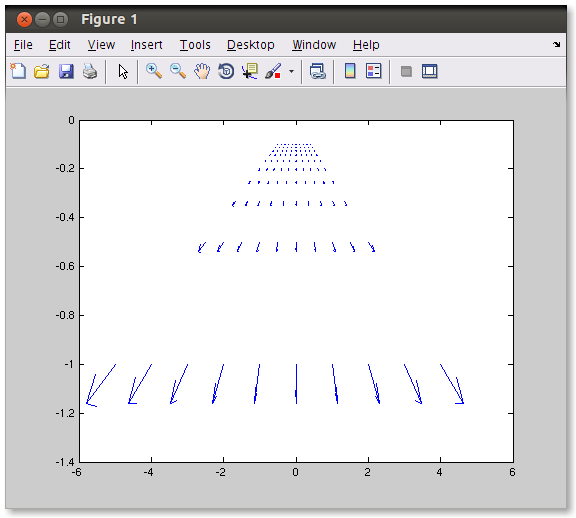
\includegraphics[width=240px]{../img/q1-a}
\end{array}$

\item[b)]
$\begin{array}{l}
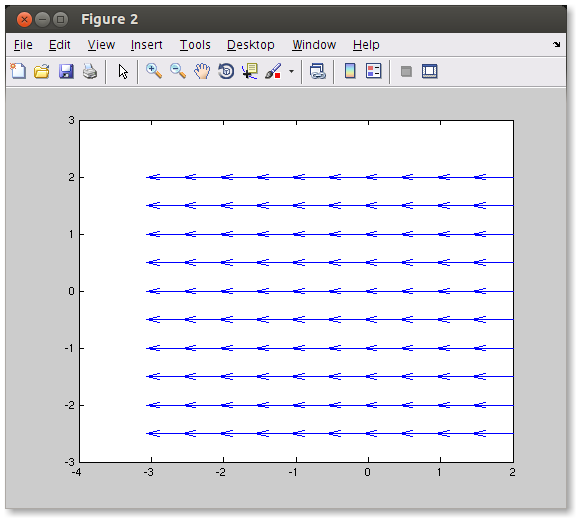
\includegraphics[width=240px]{../img/q1-b}
\end{array}$

\item[c)]
$\begin{array}{l}
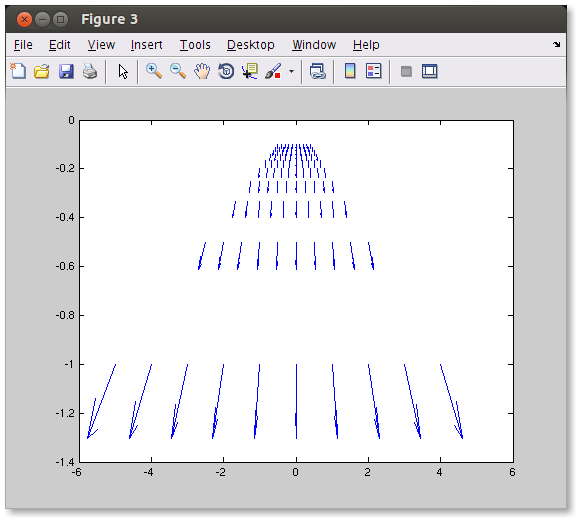
\includegraphics[width=240px]{../img/q1-c}
\end{array}$

\item[d)]
$\begin{array}{l}
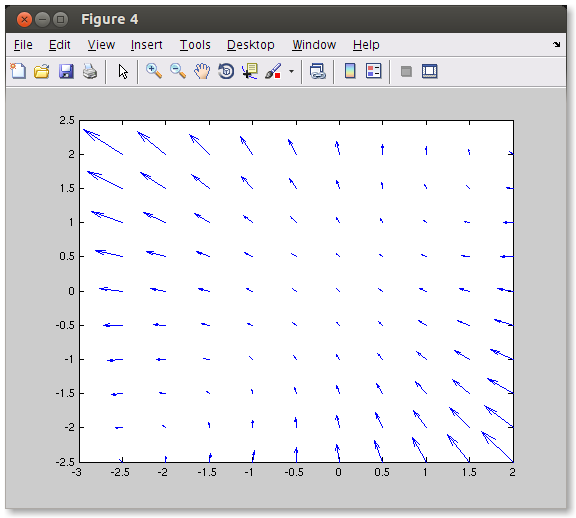
\includegraphics[width=240px]{../img/q1-d}
\end{array}$

\end{enumerate}

\newpage

\item
\begin{enumerate}
\item[1.]
First, we calculate $d$ in terms of $b, f, Z$.

\begin{align*}
Z &= \frac{bf}{d} \\
d &= \frac{bf}{Z} \\
\end{align*}

Next, we can calculate $\delta Z$ in terms of $Z, \delta d$.
\begin{align*}
Z + \delta Z &= \frac{bf}{d + \delta d} \\
Z + \delta Z &= \frac{bf}{\frac{bf}{Z} + \delta d} \\
Z + \delta Z &= \frac{bfZ}{\frac{bf} + (\delta d) Z} \\
\delta Z &= \frac{bfZ - bfZ + (\delta d) Z^2}{bf + (\delta d) Z} \\
\delta Z &= \frac{(\delta d) Z^2}{bf + (\delta d) Z} \\
\end{align*}

To calculate $\delta d$, we can use the equation above to get an equation for
$\delta d$. Rearranging the terms, we get

\begin{align*}
\delta d = \frac{\delta Z * bf}{Z^2 + Z \delta Z}
\end{align*}

From here, the code is relatively simple:
\begin{verbatim}
deltad = (err * b * f) ./ (z .* (z + err));
\end{verbatim}

\end{enumerate}

\end{enumerate}
\end{document}
